\ifx\wholebook\relax \else
% ------------------------

\documentclass[b5paper]{ctexart}
\usepackage[nomarginpar
  %, margin=.5in
]{geometry}

\addtolength{\oddsidemargin}{-0.05in}
\addtolength{\evensidemargin}{-0.05in}
\addtolength{\textwidth}{0.1in}
\usepackage[cn]{../../prelude}

\setcounter{page}{1}

\begin{document}

\title{选择排序}

\author{刘新宇
\thanks{{\bfseries 刘新宇 } \newline
  Email: liuxinyu95@gmail.com \newline}
  }

\maketitle
\fi

\markboth{选择排序}{基本算法}

\ifx\wholebook\relax
\chapter{选择排序}
\numberwithin{Exercise}{chapter}
\fi

\section{简介}
\label{introduction} \index{选择排序}
\lstset{frame = single}

我们此前介绍了插入排序。本章介绍另一种直观的排序方法―选择排序。它在性能上不如快速排序和归并排序等分治算法。我们给出选择排序性能的简要分析,并且从不同的角度加以改进,最终演进到堆排序,从而达到基于比较的排序算法性能上限$O(n \lg n)$。选择排序的思想可以在日常生活中找到。观察孩子们吃葡萄时,会发现两种类型的吃法:一种属于“乐观型”,每次吃掉最大的一颗;另一种属于“悲观型”,每次总吃掉最小的一颗。第一种孩子实际上按照由大到小的顺序吃葡萄;第二种按照由小到大的顺序吃葡萄。实际上,孩子们把葡萄按照大小进行了选择排序。选择排序的算法描述为:

\begin{enumerate}
\item 如果序列为空,排序结果也为空;
\item 否则,找到最小的元素,将其附加到结果的后面。
\end{enumerate}

这一算法产生升序结果。如果每次选择最大的元素,则结果是降序的。我们可以用抽象的比较操作实现排序。

\be
\begin{array}{rcl}
sort\ [\ ]  & = & [\ ] \\
sort\ A & = & m : sort\ (A - [m]) \quad \text{其中}\ m = min\ A
\end{array}
\ee

其中$A - [m]$是从序列$A$中去除元素$m$后的剩余部分。对应的命令式描述为:

\begin{algorithmic}[1]
\Function{Sort}{$A$}
  \State $X \gets [\ ]$
  \While{$A \neq [\ ]$}
    \State $x \gets$ \Call{Min}{$A$}
    \State \Call{Del}{$A, x$}
    \State \Call{Append}{$X, x$}
  \EndWhile
  \State \Return $X$
\EndFunction
\end{algorithmic}

\begin{figure}[htbp]
  \centering
  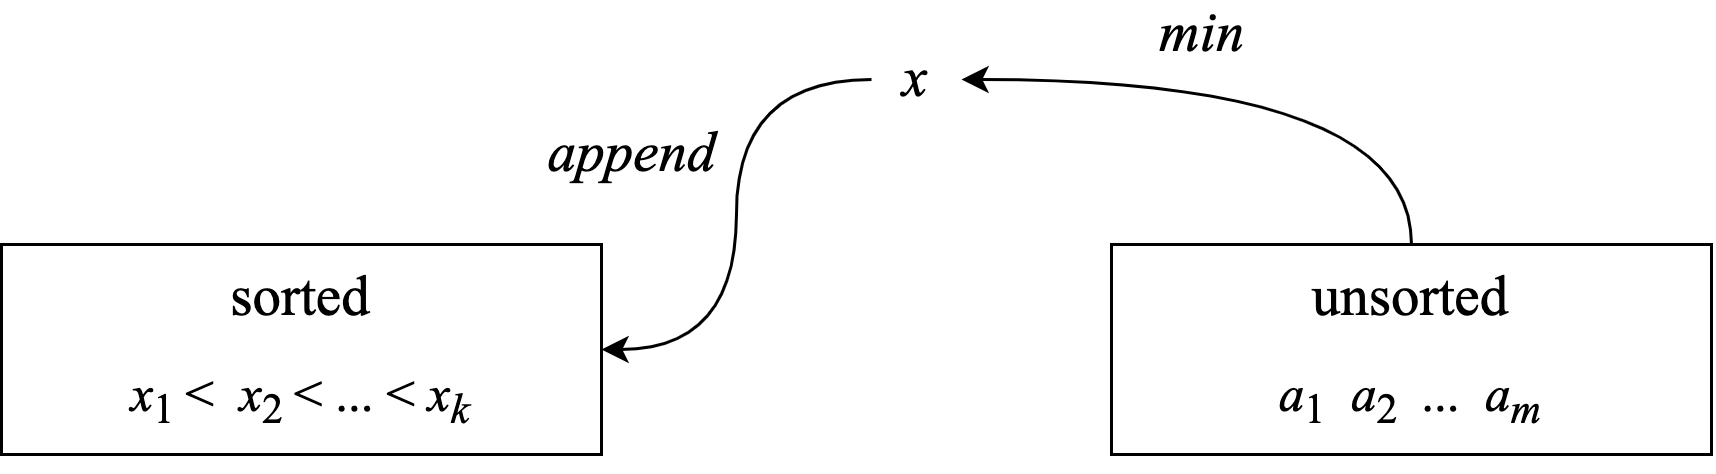
\includegraphics[scale=0.8]{img/ssort}
  \caption{左侧部分为已序元素,不断从剩余部分选择最小元素附加在左侧尾部}
  \label{fig:sel-sort}
\end{figure}

图\ref{fig:sel-sort}描述了选择排序的过程。作为改进,我们可以在$A$中进行原地排序,去掉列表$X$。将最小的元素保存在$A[1]$,将次小的元素保存在$A[2]$……。可以通过交换位置实现这一改进:当找到第$i$小的元素后,将它和$A[i]$交换。

\begin{algorithmic}[1]
\Function{Sort}{$A$}
  \For{$i \gets 1$ to $|A|$}
    \State $m \gets$ \Call{Min-At}{$A, i$}
    \State \textproc{Exchange} $A[i] \leftrightarrow A[m]$
  \EndFor
\EndFunction
\end{algorithmic}

令$A = [a_1, a_2, ..., a_n]$,当处理第$i$个元素时,$[a_1, a_2, ..., a_{i-1}]$都已排序。我们找到$[a_i, a_{i+1}, ..., a_n]$中的最小元素,将其和$a_i$交换,这样第$i$个位置就保存了正确的元素。重复这一过程直到最后一个元素。图\ref{fig:in-place-ssort}描述了这一思路。

\begin{figure}[htbp]
  \centering
  \begin{tikzpicture}[scale=0.8]
    \draw (0, 0) rectangle (3.5,1) node[pos=.5] {...已序元素...};
    \draw (4, 0) rectangle (5, 1) node (x) [pos=.5] {$x$};
    \draw (5, 0) rectangle (6, 1) node[pos=.5] {...};
    \draw (6, 0) rectangle (7, 1) node (min) [pos=.5] {$min$};
    \draw (7, 0) rectangle (8, 1) node[pos=.5] {...};
    \draw[thick, <->] (x) edge[bend left=45] node [above] {交换} (min);
  \end{tikzpicture}
  \caption{左侧部分为已序元素,不断从剩余部分找到最小的交换到正确位置}
  \label{fig:in-place-ssort}
\end{figure}

\section{查找最小元素}
\index{选择排序!查找最小元素}

为了在一组元素中寻找最小值,我们既可以用比较——交换的方式,也可以用递归的方式。在比较——交换时,令元素编号为$1, 2, ..., n$。比较编号为1,2的两个元素,选择较小的留下与编号为3的元素比较……重复这一步骤直到第$n$号元素。这一方法适合处理数组。

\begin{algorithmic}[1]
\Function{Min-At}{$A, i$}
  \State $m \gets i$
  \For{$i \gets m + 1 $ to $|A|$}
    \If{$A[i] < A[m]$}
      \State $m \gets i$
    \EndIf
  \EndFor
  \State \Return $m$
\EndFunction
\end{algorithmic}

\textproc{Min-At}查找片断$A[i...]$中最小元素的位置$m$。令$m$指向第一个元素$A[i]$,并逐一检查元素$A[i+1], A[i+2], ...$。

\index{选择排序!递归查找最小元素}
在一组元素$L$中递归查找时,如果$L$只含有一个元素,它就是最小元素。否则从$L$中取出一个元素$x$,然后在剩余部分中递归找到最小元素$y$。$x$、$y$中较小的一个就是最终的最小元素。

\be
\begin{array}{rcl}
min\ [x] & = & (x, [\ ]) \\
min\ (x:xs) & = & \begin{cases}
  x < y: & (x, xs),\ \text{其中}:\ (y, ys) = min\ xs \\
  \text{否则}: & (y,\ x:ys)
\end{cases}
\end{array}
\ee

可以进一步用尾递归优化。将全部元素分成两组:$A$、$B$。开始时$A$为空($[\ ]$),$B$包含全部元素。我们从$B$中任选两个元素比较,将较大的放入$A$,而留下较小的记为$m$。此后不断从$B$中任取一个元素,和$m$对比直到$B$变成空。这时,$m$就是最小的元素。在任何时候有不变关系:$L = A \doubleplus [m] \doubleplus B$,其中$a \leq m \leq b, a \in A, b \in B$。

\be
min\ (x:xs) = min'\ [\ ]\ x\ xs
\ee

其中:

\be
\begin{array}{rcl}
min'\ as\ m\ [\ ] & = & (m, A) \\
min'\ as\ m\ (b:bs) & = & \begin{cases}
  b < m: & min'\ (m:as)\ b\ bs \\
  \text{否则}: & min'\ (b:as)\ m\ bs \\
\end{cases}
\end{array}
\ee

函数$min$返回一对值:最小元素和剩余元素列表。这样选择排序就可以实现为:

\be
\begin{array}{rcl}
sort\ [\ ] & = & [\ ] \\
sort\ xs   & = & m : (sort\ xs'),\ \text{其中}:\ (m, xs') = min\ xs \\
\end{array}
\ee

\subsection{选择排序的性能}

选择排序在每轮中检查所有未排好的元素以挑选出最小值;总共进行了$n$次挑选,$n + (n-1) + (n-2) + ... + 1$次比较,时间复杂度为$O(\dfrac{n(n+1)}{2}) = O(n^2)$。和插入排序相比,选择排序在最好、最差和平均情况下的性能是相同的,而插入排序在最好情况下性能为线性时间$O(n)$(元素存储在一个链表中,并且顺序为逆序),最差情况下性能为平方时间$O(n^2)$。

\begin{Exercise}
\Question{下面的尾递归查找最小值实现有何问题?
\[
\begin{array}{rcl}
min'\ as\ m\ [\ ] & = & (m, A) \\
min'\ as\ m\ (b:bs) & = & \begin{cases}
  b < m: & min'\ (as \doubleplus [m])\ b\ bs \\
  \text{否则}: & min'\ (as \doubleplus [b])\ m\ bs \\
\end{cases}
\end{array}
\]
}
\Question{实现非原地和原地的选择排序程序。}
\end{Exercise}

\begin{Answer}
\Question{这里需要用链接而不是追加。追加操作的复杂度是线性的,和序列的长度成正比,而链接是常数时间的。}
\Question{实现非原地和原地的选择排序程序。TO-DO}
\end{Answer}

\section{改进}

为了支持升序、降序、和不同的比较,我们可以将比较操作抽出作为参数$\lhd$。

\be
\begin{array}{rcl}
sortBy \lhd\ [\ ] & = & [] \\
sortBy \lhd\ xs & = & m : sortBy\ \lhd\ xs',\ \text{其中}:\ (m, xs') = minBy\ \lhd\ xs \\
\end{array}
\ee

“最小值”也相应地使用传入的$\lhd$进行比较:

\be
\begin{array}{rcl}
minBy\ \lhd\ [x] & = & (x, [\ ]) \\
minBy\ \lhd\ (x:xs) & = & \begin{cases}
  x \lhd y: & (x, xs),\ \text{其中}:\ (y, ys) = minBy\ xs \\
  \text{否则}: & (y,\ x:ys)
\end{cases}
\end{array}
\ee

对于一组整数,传入小于号得到升序结果:$sortBy\ (<)\ [3, 1, 4, ...]$。这里要求比较$\lhd$操作满足严格弱序\cite{wiki-sweak-order}条件:

\begin{itemize}
\item 非自反性:对任何$x$,$x < x$不成立;
\item 非对称性:对任何$x$、$y$,若$x < y$,则$y < x$不成立;
\item 传递性:对任何$x$、$y$、$z$,若$x < y$且$y < z$,则$x < z$。
\end{itemize}

命令式原地选择排序遍历了所有的元素,可以把最小值查找实现为一个内重循环,从而使程序变得更加紧凑:

\begin{algorithmic}[1]
\Procedure{Sort}{$A$}
  \For{ $i \gets 1$ to $|A|$}
    \State $m \gets i$
    \For{$j \gets i+1$ to $|A|$}
      \If{$A[i] < A[m]$}
        \State $m \gets i$
      \EndIf
    \EndFor
    \State \textproc{Exchange} $A[i] \leftrightarrow A[m]$
  \EndFor
\EndProcedure
\end{algorithmic}

当前$n-1$个元素排好后,最后剩下的一个元素,必然是第$n$大的。因此无需再进行一次最小值查找。这样外重循环的次数可以减少一次变成$n-1$。另外,如果第$i$大的元素恰好是$A[i]$,我们无需进行交换操作。这样可以进一步改进为:

\begin{algorithmic}[1]
\Procedure{Sort}{$A$}
  \For{ $i \gets 1$ to $|A|-1$}
    \State $m \gets i$
    \For{$j \gets i+1$ to $|A|$}
      \If{$A[i] < A[m]$}
        \State $m \gets i$
      \EndIf
    \EndFor
    \If{$m \neq i$}
      \State \textproc{Exchange} $A[i] \leftrightarrow A[m]$
    \EndIf
  \EndFor
\EndProcedure
\end{algorithmic}

\subsection{鸡尾酒排序}
\index{鸡尾酒排序}

高德纳给出了另一种选择排序的实现\cite{TAOCP}。每次不是查找最小元素,而是最大元素,将其放在末尾位置。如图\ref{fig:knuth-ssort}所示,任何时候,最右侧的元素都是已序的。算法扫描未排序元素,定位到其中的最大值,然后交换到未排序部分的末尾。

\begin{algorithmic}[1]
\Procedure{Sort'}{$A$}
  \For{ $i \gets |A|$ down-to $2$}
    \State $m \gets i$
    \For{$j \gets 1$ to $i-1$}
      \If{$A[m] < A[i]$}
        \State $m \gets i$
      \EndIf
    \EndFor
    \State \textproc{Exchange} $A[i] \leftrightarrow A[m]$
  \EndFor
\EndProcedure
\end{algorithmic}

\begin{figure}[htbp]
  \centering
  \begin{tikzpicture}[scale=0.8]
    \draw (5, 0) rectangle (6, 1) node[pos=.5] {...};
    \draw (6, 0) rectangle (7, 1) node (max) [pos=.5] {$max$};
    \draw (7, 0) rectangle (8, 1) node[pos=.5] {...};
    \draw (8, 0) rectangle (9, 1) node (x) [pos=.5] {$x$};
    \draw (10,0) rectangle (13.5,1) node[pos=.5] {...已序元素...};
    \draw[thick, <->] (x) edge[bend right=45] node [above] {交换} (max);
  \end{tikzpicture}
  \caption{每次选择最大的元素放到末尾}
  \label{fig:knuth-ssort}
\end{figure}

每次选择最大的元素也可以实现升序排序。进一步,每次扫描可以同时查找最小值和最大值,分别将最小值放到开头,将最大值放到末尾。这样可以将外重循环次数减半。这一算法称为“鸡尾酒排序”。如图\ref{fig:cock-tail-sort}所示,任何时候,左侧和右侧部分都包含了已序元素。算法扫描未排序的部分,定位到最小和最大的两个元素,然后分别将它们交换到开头和末尾。

\begin{algorithmic}[1]
\Procedure{Sort}{$A$}
  \For{$i \gets 1 $ to $\lfloor \dfrac{|A|}{2} \rfloor$}
    \State $min \gets i$
    \State $max \gets |A| + 1 - i$
    \If{$A[max] < A[min]$}
      \State \textproc{Exchange} $A[min] \leftrightarrow A[max]$
    \EndIf
    \For{$j \gets i + 1$ to $|A| - i$}
      \If{$A[j] < A[min]$}
        \State $min \gets j$
      \EndIf
      \If{$A[max] < A[j]$}
        \State $max \gets j$
      \EndIf
    \EndFor
    \State \textproc{Exchange} $A[i] \leftrightarrow A[min]$
    \State \textproc{Exchange} $A[|A|+1-i] \leftrightarrow A[max]$
  \EndFor
\EndProcedure
\end{algorithmic}

\begin{figure}[htbp]
  \centering
  \begin{tikzpicture}[scale=0.8]
    \draw (0,0) rectangle (3.5,1) node[pos=.5] {...已序较小元素...};
    \draw (4, 0) rectangle (5, 1) node (x) [pos=.5] {$x$};
    \draw (5, 0) rectangle (6, 1) node[pos=.5] {...};
    \draw (6, 0) rectangle (7, 1) node (max) [pos=.5] {$max$};
    \draw (7, 0) rectangle (8, 1) node[pos=.5] {...};
    \draw (8, 0) rectangle (9, 1) node (min) [pos=.5] {$min$};
    \draw (9, 0) rectangle (10, 1) node[pos=.5] {...};
    \draw (10, 0) rectangle (11, 1) node (y) [pos=.5] {$y$};
    \draw (12,0) rectangle (15.5,1) node[pos=.5] {...已序较大元素...};
    \draw[thick, <->] (x) edge[bend right=45] node [below] {交换} (min);
    \draw[thick, <->] (y) edge[bend right=45] node [above] {交换} (max);
  \end{tikzpicture}
  \caption{一次扫描同时定位出最小和最大元素,然后将它们放到正确的位置}
  \label{fig:cock-tail-sort}
\end{figure}

注意,在内重循环开始前,如果最右侧的元素小于最左侧的元素,需要将它们交换。这是因为我们的扫描范围不包括两端上的元素。也可以用递归的方式实现鸡尾酒排序:

\begin{enumerate}
  \item 若待排序的序列为空或者仅含有一个元素,排序结果为原序列;
  \item 否则,找到最小和最大值,分别放到开头和结尾位置,然后递归地将剩余元素排序。
\end{enumerate}

\be
\begin{array}{rcl}
sort\ [\ ] & = & [\ ] \\
sort\ [x] & = & [x] \\
sort\ xs & = & a : (sort\ xs') \doubleplus [b], {其中}: (a, b, xs') = \textit{minMax}\ xs \\
\end{array}
\ee

其中,函数\textit{minMax}从序列中抽取出最小值和最大值:

\be
\textit{minMax}\ (x:y:xs) = foldr\ sel (min\ x\ y, max\ x\ y, [\ ])\ xs
\ee

我们选取头两个元素分别作为已找到的最小值$x_0$,最大值$x_1$,用$foldr$扫描序列,其中$sel$定义为:

\[
sel\ x\ (x_0, x_1, xs) = \begin{cases}
  x < x_0: & (x, x_1, x_0 : xs) \\
  x_1 < x: & (x_0, x, x_1 : xs) \\
  \text{否则}: & (x_0, x_1, x : xs) \\
\end{cases}
\]

尽管\textit{minMax}的时间性能是线性时间$O(n)$的,但$\doubleplus[b]$的代价较大。如图\ref{fig:cock-tail-sort}所示,令左侧$A$包含较小的已序元素;右侧$B$包含较大的已序元素。用$A$和$B$作为累积器,可以将鸡尾酒排序转换为尾递归的:

\be
\begin{array}{rcl}
sort'\ A\ B\ [\ ] & = & A \doubleplus B \\
sort'\ A\ B\ [x]  & = & A \doubleplus (x:B) \\
sort'\ A\ B\ (x:xs) & = & sort'\ (A \doubleplus [x_0])\ xs'\ (x_1:B) \\
\end{array}
\ee

其中:$(x_0, x_1, xs') = \textit{minMax}\ xs$,我们传入空的$A$、$B$启动排序:$sort = sort'\ [\ ]\ [\ ]$。追加操作仅仅发生在$A \doubleplus [x_0]$;而$x_1$则被链结到$B$的前面。每次递归都会产生一次追加操作。为了消除它,我们可以将$A$保存为逆序$\overleftarrow{A}$,这样就可以将$x_0$链结到前面而不是追加。我们有如下等价关系:

\be
\begin{array}{rcl}
A' & = & A \doubleplus [x] \\
   & = & reverse\ (x : reverse\ A) \\
   & = & reverse\ (x : \overleftarrow{A}) \\
   & = & \overleftarrow{ x : \overleftarrow{A}}
\end{array}
\ee

最后执行一次反转操作将$\overleftarrow{A'}$转换回$A'$。根据这一思路,可进一步改进如下:

\be
\begin{array}{rcl}
sort'\ A\ B\ [\ ] & = & (reverse\ A) \doubleplus B \\
sort'\ A\ B\ [x]  & = & (reverse\ x:A) \doubleplus B \\
sort'\ A\ B\ (x:xs) & = & sort'\ (x_0:A)\ xs'\ (x_1:B) \\
\end{array}
\ee

\section{继续改进}

虽然鸡尾酒排序将循环次数减半,但时间复杂度仍然是$O(n^2)$的。通过比较进行排序,需要检查元素间的大小顺序,外重循环是必须的。为了选出最小元素,必须每次都扫描全部元素么?在查找第一个最小元素时,我们实际遍历了序列,知道哪些元素相对较小,哪些相对较大。但在查找后继的最小元素时,我们没有复用关于相对大小的信息,而是从头开始再次遍历。进一步改进的关键在于重用已有的结果。其中一种方法是来自体育竞赛。

\subsection{锦标赛淘汰法}
\index{锦标赛淘汰法}

足球世界杯每四年举办一次。来自各个大洲的32支球队最终进入决赛。1982年前,决赛阶段只有16支球队\cite{wiki-wc}。我们回到1978年,并且想像一种特殊的方法来决定冠军:在第一轮比赛中,所有参赛球队被分为8组进行比赛;比赛产生8支获胜球队,其余8支被淘汰。接下来,在第二轮比赛中,8支球队被分成4组。比赛产生4支获胜球队;然后这4支球队分成两对,比赛产生最终的两支球队争夺冠军。经过4轮比赛,冠军就可产生。总共的比赛场次为:$8+4+2+1 = 15$。但是我们并不满足仅仅知道谁是冠军,我们还想知道哪支球队是亚军。有人会问最后一场比赛中被冠军击败的队伍不是亚军么?在真实的世界杯中,的确如此。但是这个规则在某种程度上并不公平。我们常常听说过“死亡之组”,假设巴西队一开始就和德国队进行比赛。虽然它们两个都是强队,但是必须有一支在一上来就被淘汰。这支被淘汰的球队,很可能会打败除冠军外的其他所有球队。图\ref{fig:tournament-tree-1}描述了这一情况。

\begin{figure}[htbp]
  \centering
  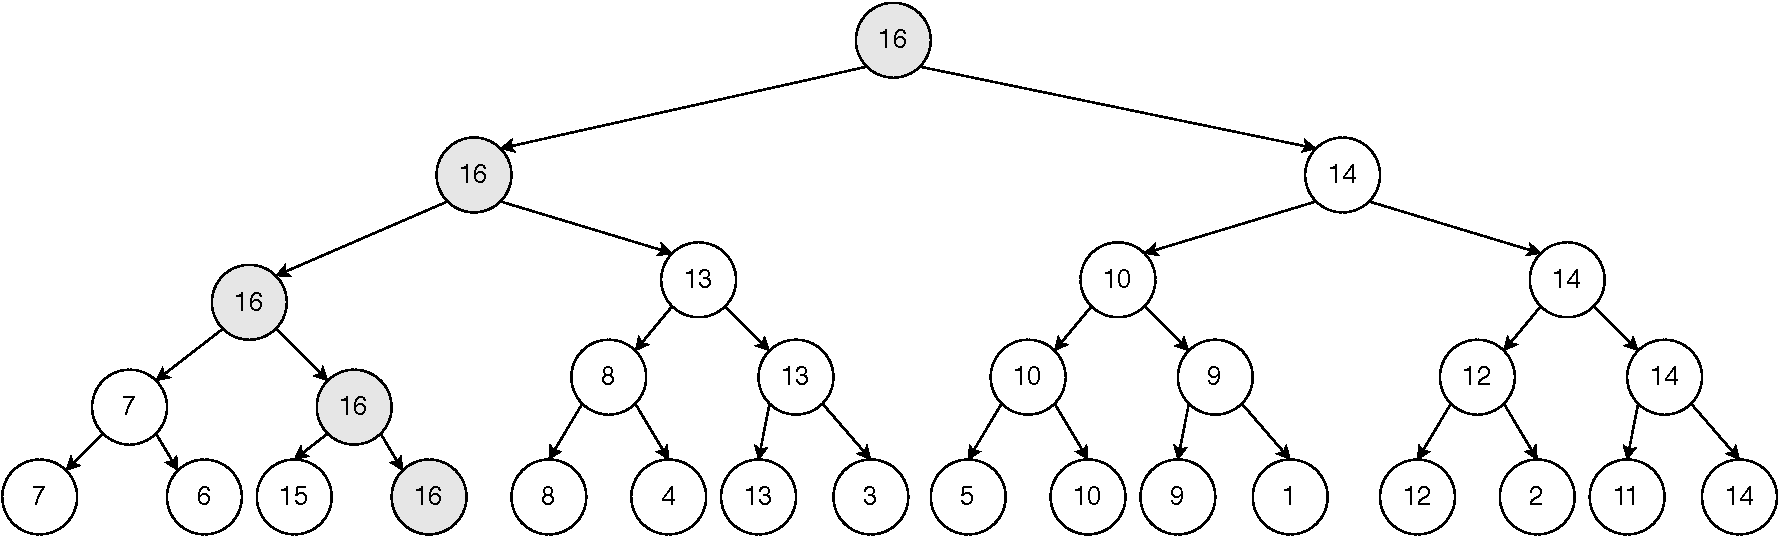
\includegraphics[scale=0.28]{img/tournament-tree-1}
  \caption{元素15在第一轮就被淘汰}
  \label{fig:tournament-tree-1}
\end{figure}

每支队伍有一个代表其实力的数字。数字越大,实力越强。假设数字较大的队永远会战胜数字较小的队(虽然现实中不会这样)。代表冠军的数字为16,根据假设的规则,数字14不是亚军,而是在第一轮就被淘汰的15。我们需要一种快速的方法在锦标赛树中找到第二大值。此后,我们只要不断重复这一方法,逐一找出第三大,第四大……就可以完成基于选择的排序。我们可以把冠军的数字更改成一个很小的值(例如$-\infty$),这样以后它就不会被选中,这样第二名就会成为新的冠军。假设有$2^m$支球队,$m$是自然数,仍然需要$2^{m-1} + 2^{m-2} + ... + 2 + 1 = 2^m-1$次比较才能产生新的冠军,这和第一次寻找冠军花费的代价相同。实际上,我们无需再进行自底向上的比较。锦标赛树中保存了足够的顺序信息。实力第二强的队,一定在某个时刻被冠军击败,否则它就会是最终的冠军。因此我们可以从锦标赛树的根节点出发,沿着产生冠军的路径向叶子方向遍历,在这条路径上寻找第二强的队。图\ref{fig:tournament-tree-1}中,这条路径被标记为灰色,需要检查的元素包括$\{14, 13, 7, 15\}$,这一思路可以描述如下:

\begin{enumerate}
\item 从待排序元素构建一棵锦标赛树,冠军(最大值)位于树根;
\item 取出树根,自顶向下沿着冠军路径将最大值替换为$-\infty$;
\item 自底向上沿着刚才的路径回溯,找出新的冠军,并将其置于树根;
\item 重复步骤2,直到所有的元素都被取出。
\end{enumerate}

\captionsetup[subfigure]{labelformat=empty, margin=10pt}
\begin{figure}[htbp]
  \centering
  \subcaptionbox{取出16,将其替换为$-\infty$,15上升为新的根}{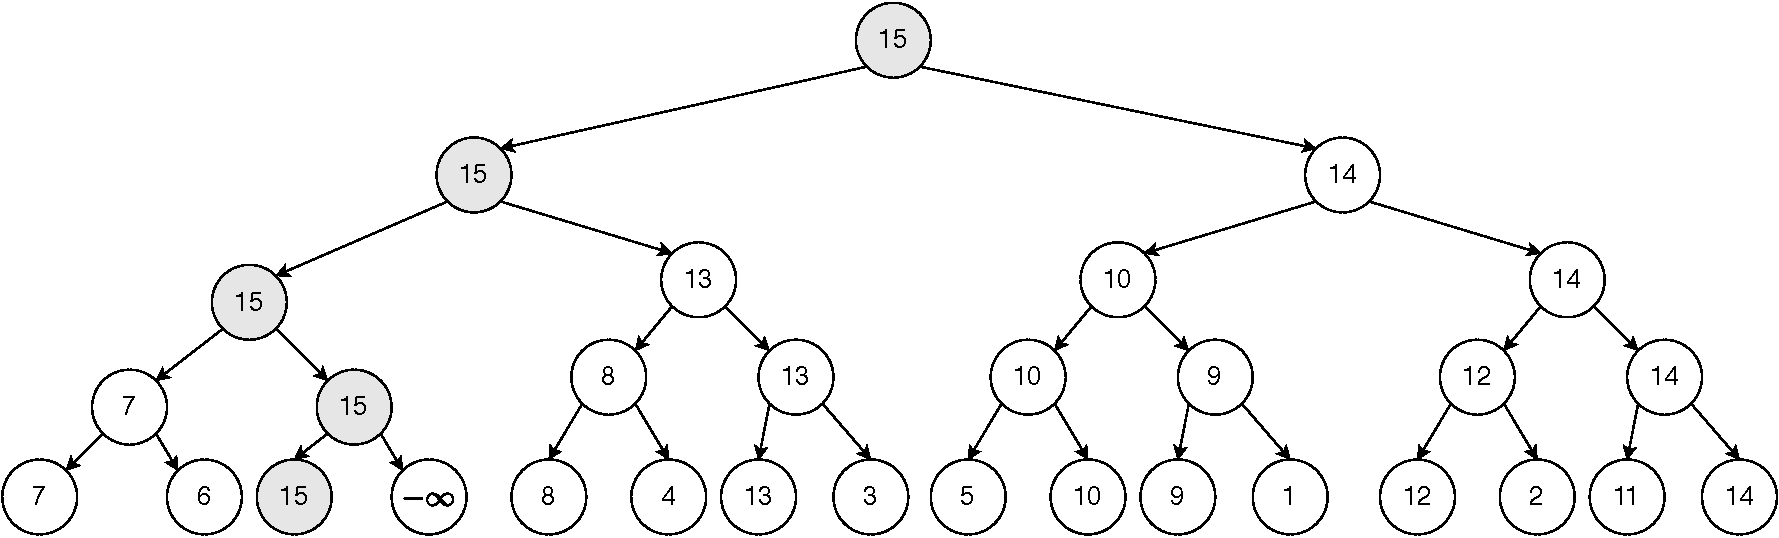
\includegraphics[scale=0.28]{img/tournament-tree-2}} \\
  \subcaptionbox{取出15,将其替换为$-\infty$,14上升为新的根}{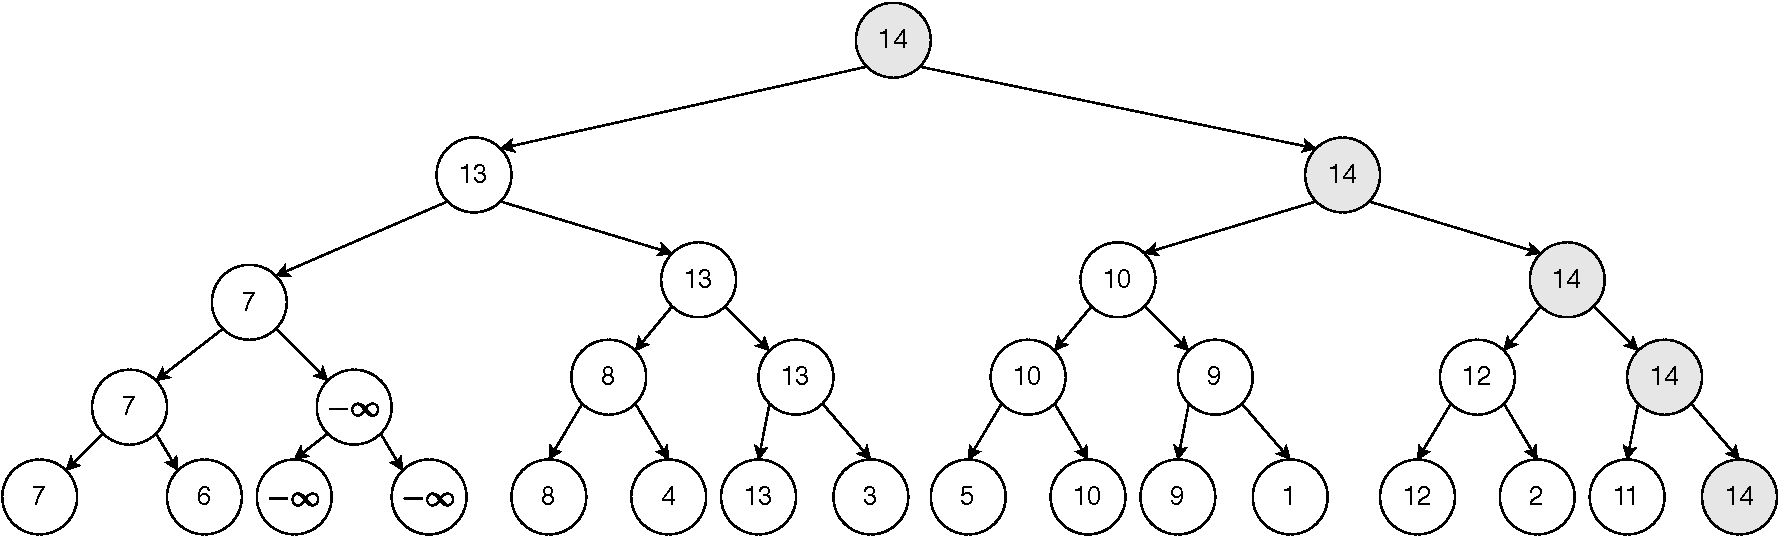
\includegraphics[scale=0.28]{img/tournament-tree-3}} \\
  \subcaptionbox{取出14,将其替换为$-\infty$,13上升为新的根}{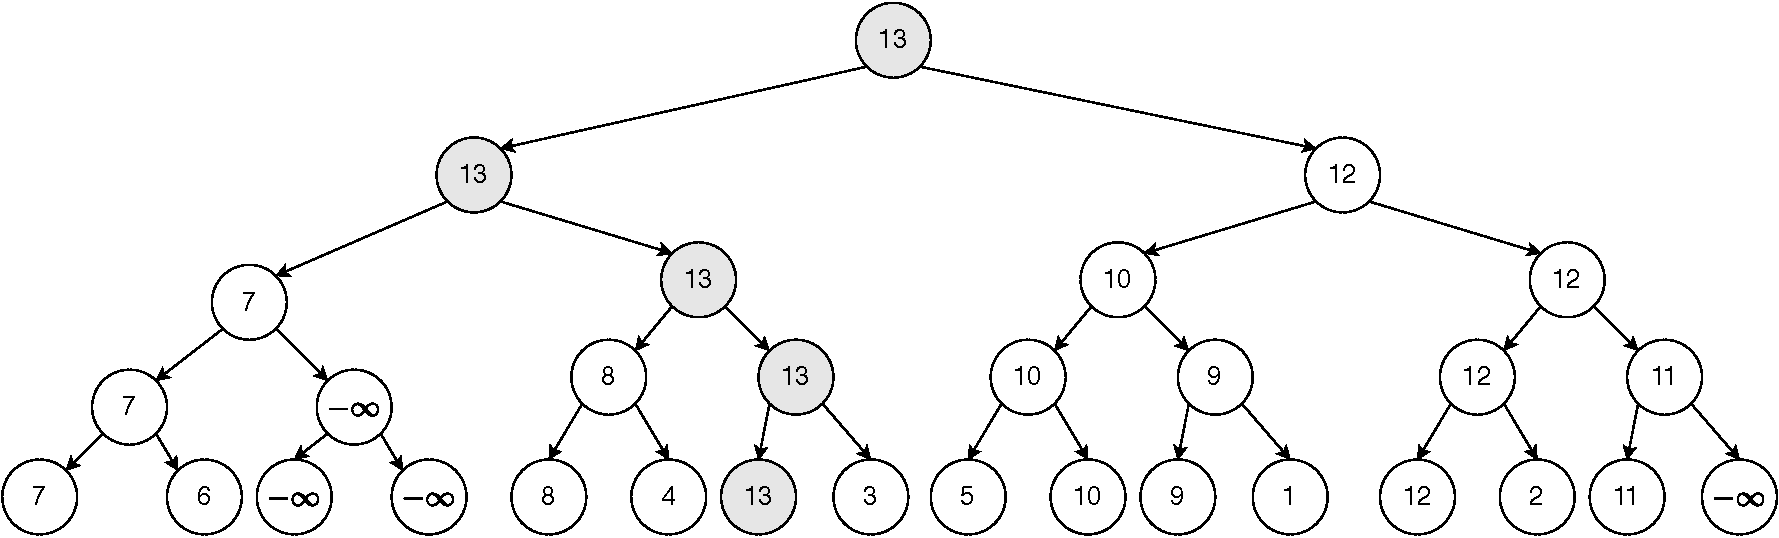
\includegraphics[scale=0.28]{img/tournament-tree-4}}
  \caption{锦标赛树排序的前几步}
  \label{fig:tournament-tree-4}
\end{figure}
\captionsetup[subfigure]{labelformat=parens}

为了对一组元素排序,我们先从它们构造一棵锦标赛树,然后不断取出冠军,图\ref{fig:tournament-tree-4}给出了这一排序的前几个步骤。我们可以复用二叉树的定义来表示锦标赛树,为了方便自底向上回溯,每个节点需要指向它的父节点。元素数目$n$可能不是恰好$2^m$个。两两比较后,可能剩余元素没有“对手”,而“轮空”直接进入下一轮比赛。为了构造锦标赛树,我们从每个元素构造一棵单一叶子节点的树,这样就得到了$n$棵二叉树。然后我们每次取出两棵树$t_1$、$t_2$,构造出一棵更大的二叉树$t$。其中$t$的根为$max(key(t_1), key(t_2))$,左右子树为$t_1$、$t_2$。重复这一步骤可以得到一组新的树,每棵新树的高度增加了1,如有剩余则进入下一轮。这样一轮过后,树减半为$\lfloor \dfrac{n}{2} \rfloor$。持续同样的操作最终得到一棵锦标赛树。总时间复杂度为$O(n + \dfrac{n}{2} + \dfrac{n}{4} + ... ) = O(2n) = O(n)$。

\begin{algorithmic}[1]
\Function{Build-Tree}{$A$}
  \State $T \gets [\ ]$
  \For{each $x \in A$}
    \State \textproc{Append}($T$, \Call{Node}{NIL, $x$, NIL})
  \EndFor
  \While{$|T| > 1$}
    \State $T' \gets [\ ]$
    \For{every $t_1, t_2 \in T$}
      \State $k \gets$ \textproc{Max}(\Call{Key}{$t_1$}, \Call{Key}{$t_2$})
      \State \textproc{Append}($T'$, \Call{Node}{$t_1$, $k$, $t_2$})
    \EndFor
    \If{|T| is odd}
      \State \textproc{Append}($T'$, \Call{Last}{$T$})
    \EndIf
    \State $T \gets T'$
  \EndWhile
  \State \Return $T[1]$
\EndFunction
\end{algorithmic}

每次取出锦标赛树的根节点后,我们自顶向下将其替换为$-\infty$,然后在通过父节点向上回溯,找出新的最大值。

\begin{algorithmic}[1]
\Function{Pop}{$T$}
  \State $m \gets$ \Call{Key}{$T$}
  \State \Call{Key}{$T$} $\gets -\infty$
  \While{$T$ is not leaf}  \Comment{自顶向下将$m$替换为$-\infty$}
    \If{\textproc{Key}(\Call{Left}{$T$}) $ = m$}
      \State $T \gets$ \Call{Left}{$T$}
    \Else
      \State $T \gets$ \Call{Right}{$T$}
    \EndIf
    \State \Call{Key}{$T$} $\gets -\infty$
  \EndWhile
  \While{\Call{Parent}{$T$} $\neq$ NIL} \Comment{自底向上决出新冠军}
    \State $T \gets$ \Call{Parent}{$T$}
    \State \Call{Key}{$T$} $\gets$ \textproc{Max}(\textproc{Key}(\Call{Left}{$T$}), \textproc{Key}(\Call{Right}{$T$}))
  \EndWhile
  \State \Return $(m, T)$ \Comment{返回最大元素和更新的树}
\EndFunction
\end{algorithmic}

\textproc{Pop}上下处理两遍,自顶向下一遍,接着自底向上沿着“冠军之路”一遍。由于锦标赛树是平衡的,路径的长度,也就是树的高度为$O(\lg n)$。时间复杂度为$O(\lg n)$。下面是锦标赛排序的实现。算法首先用$O(n)$时间构建一棵锦标赛树,然后执行$n$次弹出操作,逐一从树中取出最大值。每次弹出操作的性能为$O(\lg n)$,锦标赛排序的总时间复杂度为$O(n \lg n)$。

\begin{algorithmic}[1]
\Procedure{Sort}{$A$}
  \State $T \gets$ \Call{Build-Tree}{$A$}
  \For{$i \gets |A|$ down to $1$}
    \State $(A[i], T) \gets$ \Call{Pop}{$T$}
  \EndFor
\EndProcedure
\end{algorithmic}

\subsubsection{递归锦标赛排序}

锦标赛淘汰法也可以用纯函数式的方式实现。我们会看到弹出操作中的两遍处理过程(第一遍自顶向下将冠军替换为$-\infty$;第二遍自底向上查找新的冠军)可以通过递归合并起来。于是不再需要存储父节点的引用。我们可以复用函数式的二叉树定义,如下面的例子Haskell代码所示:

\lstset{language=Haskell}
\begin{lstlisting}[style=Haskell]
data Tr a = Empty | Br (Tr a) a (Tr a)
\end{lstlisting}

一棵二叉树或者为空,或者为一个分支节点,包含一个key和左右子树。每棵子树都是一棵二叉树。

此前,我们使用一个较大的负整数来表示$-\infty$。但是这个方法是临时性的,有诸多不便。某些编程环境支持代数类型,这样就可以明确定义负无穷。例如下面的Haskell程序建立了无穷的定义\footnote{如果希望直接使用默认的\texttt{Ord}来比较大小,则需要按照负无穷、普通数字和正无穷的顺序来声明。当然,也可以将我们的类型声明为\texttt{Ord}的一个instance,然后给出大小比较的规则。这些是语言特有的性质,超出了本书的范围。读者可以参考其他Haskell资料}.。

\lstset{language=Haskell}
\begin{lstlisting}[style=Haskell]
data Infinite a = NegInf | Only a | Inf deriving (Eq, Ord)
\end{lstlisting}

接下来的部分,我们使用$min()$函数来决定比赛的胜者,相应的锦标赛树选择最小的元素作为冠军。

记函数$key(T)$返回树$T$根节点的key。函数$wrap(x)$将元素$x$装入一个叶子节点。函数$tree(l, k, r)$构造一个分支节点。其中$k$是key,$l$和$r$分别是左右分支。

在淘汰过程中,我们比较两棵树,选择较小的key作为新节点的key,进行比较的两棵树作为左右子树。

\be
branch(T_1, T_2) = tree(T_1, min(key(T_1), key(T_2)), T_2)
\ee

对应的Haskell例子代码为:

\lstset{language=Haskell}
\begin{lstlisting}[style=Haskell]
branch t1 t2 = Br t1 (min (key t1) (key t2)) t2
\end{lstlisting}

此前的锦标赛排序算法有一个限制。它要求待排序的元素个数必须是$2^m$,否则我们无法构造一棵完全二叉树。现在考虑如何克服这一问题。每次我们都选出两棵树,比较并且选择较大的。如果树的总数目为偶数,我们总能不断选出两棵。在真正的足球比赛中,如果某支球队因故缺席了比赛(例如航班延误),则会有一支球队没有对手。可以规定这支球队为胜者,直接进入接下来的比赛。我们完全可以使用类似的方法。

首先将每个元素都装入叶子节点,然后开始构造锦标赛树。

\be
build(L) = build'(\{wrap(x) | x \in L\})
\ee

函数$build'(\mathbb{T})$中,如果列表$\mathbb{T}$中仅有一棵树,则此树就是最终结果。否则,它将每两棵树分成一组,然后决定胜者。如果有奇数棵树,就规定最后一棵树为胜者,可以进入下一轮比赛。然后我们递归调用这一构造算法。

\be
build'(\mathbb{T}) = \left \{
  \begin{array}
  {r@{\quad:\quad}l}
  \mathbb{T} & |\mathbb{T}| \leq 1 \\
  build'(pair(\mathbb{T})) & otherwise
  \end{array}
\right.
\ee

这一算法还能处理另外一种特殊情况:如果待排序的列表为空,则结果也为空。

如果列表中至少有两棵树,记$\mathbb{T} = \{ T_1, T_2, ...\}$,而$\mathbb{T}'$表示除最初两棵树外的剩余树。函数$pair(\mathbb{T})$定义如下:

\be
pair(\mathbb{T}) = \left \{
  \begin{array}
  {r@{\quad:\quad}l}
  \{ branch(T_1, T_2) \} \cup pair(\mathbb{T}') & |\mathbb{T}| \geq 2 \\
  \mathbb{T} & otherwise
  \end{array}
\right.
\ee

下面的Haskell例子代码给出了构造锦标赛树的完整程序。

\lstset{language=Haskell}
\begin{lstlisting}[style=Haskell]
fromList :: (Ord a) => [a] -> Tr (Infinite a)
fromList = build . (map wrap) where
  build [] = Empty
  build [t] = t
  build ts = build $ pair ts
  pair (t1:t2:ts) = (branch t1 t2):pair ts
  pair ts = ts
\end{lstlisting} %$

为了从锦标赛树中取得冠军(最小元素),我们检查左右子树,看哪一棵子树的key和根节点的key相等。然后递归地从子树中取出冠军直到到达叶子节点。记$T$的左子树为$L$,右子树为$R$,$K$为key,弹出算法可以定义如下:

\be
pop(T) =  \left \{
  \begin{array}
  {r@{\quad:\quad}l}
  tree(\phi, \infty, \phi) & L = \phi \land R = \phi \\
  tree(L', min(key(L'), key(R)), R) & K = key(L), L' = pop(L) \\
  tree(L, min(key(L), key(R')), R') & K = key(R), R' = pop(R)
  \end{array}
\right.
\ee

下面的Haskell例子代码实现了弹出算法。

\lstset{language=Haskell}
\begin{lstlisting}[style=Haskell]
pop (Br Empty _ Empty) = Br Empty Inf Empty
pop (Br l k r) | k == key l = let l' = pop l in Br l' (min (key l') (key r)) r
               | k == key r = let r' = pop r in Br l (min (key l) (key r')) r'
\end{lstlisting}

注意这一算法仅仅将冠军元素删除而没有返回,因此有必要定义另外一个函数从根节点提取冠军元素。

\be
top(T) = key(T)
\ee

使用这些定义好的函数,锦标赛淘汰排序法可以形式化为下面的等式:

\be
sort(L) = sort'(build(L))
\ee

其中$sort'(T)$不断从锦标赛树中弹出最小的元素:

\be
sort'(T) = \left \{
  \begin{array}
  {r@{\quad:\quad}l}
  \phi & T = \phi \lor key(T) = \infty \\
  \{ top(T) \} \cup sort'(pop(T)) & otherwise
  \end{array}
\right.
\label{eq:tsort}
\ee

下面的Haskell例子程序实现了完整的锦标赛淘汰排序算法。

\lstset{language=Haskell}
\begin{lstlisting}[style=Haskell]
top = only . key

tsort :: (Ord a) => [a] -> [a]
tsort = sort' . fromList where
    sort' Empty = []
    sort' (Br _ Inf _) = []
    sort' t = (top t) : (sort' $ pop t)
\end{lstlisting} %$

其中用以支持无穷类型的辅助函数\texttt{only}、\texttt{key}和\texttt{wrap}定义如下:

\lstset{language=Haskell}
\begin{lstlisting}[style=Haskell]
only (Only x) = x
key (Br _ k _ ) = k
wrap x = Br Empty (Only x) Empty
\end{lstlisting}

\begin{Exercise}
  \begin{itemize}
    \item 实现命令式锦标赛淘汰法中的辅助函数\texttt{leaf()}、\texttt{branch}、\texttt{max()}、\texttt{isleaf()}和\texttt{release()}。
    \item 在一门支持垃圾回收(GC)的语言中实现命令式的锦标赛淘汰法排序程序。
    \item 为什么我们的锦标赛树淘汰法排序程序可以处理重复元素(元素的值相等)?如果相等元素的顺序经过排序后保持不变,我们称之为稳定排序。锦标赛树淘汰法排序是稳定排序么?
    \item 设计一个命令式的锦标赛淘汰排序算法,满足下面的条件:
      \begin{itemize}
        \item 可以处理任意数目的元素;
        \item 不使用硬编码(hard code)的大负数,可以处理任意值的元素。
      \end{itemize}
    \item 比较锦标赛树淘汰算法和二叉搜索树排序算法,分析它们的时间和空间效率。
    \item 比较堆排序算法和二叉搜索树排序算法,分析它们的时间和空间效率。
  \end{itemize}
\end{Exercise}

\subsection{使用堆排序进行最后的改进}

通过使用锦标赛树淘汰法,我们将基于选择的排序算法性能提高到$O(n \lg n)$。这已经达到了基于比较的排序算法的上限\cite{TAOCP}。但是,这里仍然有提高的空间。排序完成后,锦标赛树的所有节点都变成了负无穷,这棵完全二叉树不再含有任何有用的信息,但它却占据了很大空间。有没有办法在弹出后释放节点呢?

另外我们可以观察到,如果待排序的元素有$n$个,我们实际上使用了$2n$个节点。其中有$n$个叶子和$n$个分支。有没有办法能节约一半空间呢?

如果我们认为根节点的key为无穷,则树为空,那么上一节最后给出的公式\ref{eq:tsort}就可以进一步概括为更加通用的形式:

\be
sort'(T) = \left \{
  \begin{array}
  {r@{\quad:\quad}l}
  \phi & T = \phi\\
  \{ top(T) \} \cup sort'(pop(T)) & otherwise
  \end{array}
\right.
\ee

这和我们在上一章堆排序给出的公式完全一样。堆总是在顶部保存最小(或最大)值,并且提供了快速的弹出操作。使用数组的binary堆实际上将树结构“编码”成数组的索引,因此除了$n$个单元外,无需任何额外的空间。函数式的堆,如左偏堆和splay堆也只需要$n$个节点。我们将在下一章介绍更多种类的堆,它们在许多情况下都有很好的性能。

\section{小结}

本章我们介绍了选择排序的进化过程。选择排序简单、直观,经常被用来教授编程中的多重循环。它的结构虽然简单,但是性能却是平方级别的。本章中,我们看到,选择排序不仅可以通过细微调整加以改进,而且还可以通过改变底层的数据结构,进化到锦标赛淘汰排序和堆排序,从而在本质上得到性能的提升。

\section{附录:例子程序}

尾递归实现的选择排序:
\begin{Haskell}
sort [] = []
sort xs = x : sort xs'
  where
    (x, xs') = extractMin xs

extractMin (x:xs) = min' [] x xs
  where
    min' ys m [] = (m, ys)
    min' ys m (x:xs) = if m < x then min' (x:ys) m xs
                                else min' (m:ys) x xs
\end{Haskell}

鸡尾酒排序:

\begin{lstlisting}[language = Bourbaki]
[A] cocktailSort([A] xs) {
    Int n = length(xs)
    for Int i = 0 to n / 2 {
        var (mi, ma) = (i, n - 1 -i)
        if xs[ma] < xs[mi] then swap(xs[mi], xs[ma])
        for Int j = i + 1 to n - 1 - i {
            if xs[j] < xs[mi] then mi = j
            if xs[ma] < xs[j] then ma = j
        }
        swap(xs[i], xs[mi])
        swap(xs[n - 1 - i], xs[ma])
    }
    return xs
}
\end{lstlisting}

尾递归的鸡尾酒排序:

\begin{Haskell}
csort xs = cocktail [] [] xs
  where
    cocktail as bs []  = reverse as ++ bs
    cocktail as bs [x] = reverse (x:as) ++ bs
    cocktail as bs xs  = let (mi, ma, xs') = minMax xs
                         in cocktail (mi:as) (ma:bs) xs'

minMax (x:y:xs) = foldr sel (min x y, max x y, []) xs
  where
    sel x (mi, ma, ys) | x < mi = (x, ma, mi:ys)
                       | ma < x = (mi, x, ma:ys)
                       | otherwise = (mi, ma, x:ys)
\end{Haskell}

复用二叉树构造锦标赛树:

\begin{lstlisting}[language = Bourbaki]
Node<T> build([T] xs) {
    [T] ts = []
    for x in xs {
        append(ts, Node(null, x, null))
    }
    while length(ts) >  1 {
        [T] ts' = []
        for l, r in ts {
            append(ts', Node(l, max(l.key, r.key), r))
        }
        if odd(length(ts)) then append(ts', last(ts))
        ts = ts'
    }
    return ts[0];
}
\end{lstlisting}

从锦标赛树取出冠军:

\begin{lstlisting}[language = Bourbaki]
T pop(Node<T> t) {
    T m = t.key
    t.key = -INF
    while not isLeaf(t) {
        t = if t.left.key == m then t->left else t->right
        t.key = -INF
    }
    while (t.parent != null) {
        t = t.parent
        t.key = max(t.left.key, t.right.key)
    }
    return (m, t);
}
\end{lstlisting}

剪标赛树排序:

\begin{lstlisting}[language = Bourbaki]
void sort([A] xs) {
    Node<T> t = build(xs)
    for Int n = length(xs) - 1 downto 0 {
        (xs[n], t) = pop(t)
    }
}
\end{lstlisting}

\ifx\wholebook\relax\else
\section{参考答案}
\shipoutAnswer

\begin{thebibliography}{99}

\bibitem{TAOCP}
Donald E. Knuth. ``The Art of Computer Programming, Volume 3: Sorting and Searching (2nd Edition)''. Addison-Wesley Professional; 2 edition (May 4, 1998) ISBN-10: 0201896850 ISBN-13: 978-0201896855

\bibitem{CLRS}
Thomas H. Cormen, Charles E. Leiserson, Ronald L. Rivest and Clifford Stein.
``Introduction to Algorithms, Second Edition''. ISBN:0262032937. The MIT Press. 2001 (《算法导论》中文版)

\bibitem{wiki-sweak-order}
Wikipedia. ``Strict weak order''. \url{https://en.wikipedia.org/wiki/Strict_weak_order}

\bibitem{wiki-wc}
Wikipedia. ``FIFA world cup''. \url{https://en.wikipedia.org/wiki/FIFA_World_Cup}

\end{thebibliography}

\end{document}
\fi
